The \dword{coldata} \dword{asic} is responsible for all communication between the %cold TPC electronics 
\dword{ce} on \dwords{femb} and electronics located outside the cryostat.  The \dword{coldata} \dword{asic} is being designed by engineers from \fnal and Southern Methodist University.  Each \dword{femb} contains two \dword{coldata} \dwords{asic}.  \dword{coldata} receives command and control information; it provides clocks to the cold \dword{adc} \dwords{asic} and relays commands to the \dword{larasic} front-end and to the cold \dword{adc} \dwords{asic} to set operating modes and initiate calibration procedures.  \dword{coldata} receives data from the \dword{adc} \dwords{asic}, reformats these data, merges data streams, formats data packets, and sends these data packets to the warm electronics using \SI{1.28}{Gbps} links.  These links include line drivers with pulse pre-emphasis.  All the components of \dword{coldata}, with the exception of the line drivers and of the interface to the \dword{adc}, have been implemented in the CDP1 prototype \dword{asic} and demonstrated to work as designed both at room temperature and at \SI{77}{K}.  A block diagram of \dword{coldata} is shown in Figure~\ref{fig:coldata}.  

\begin{dunefigure}
[Block diagram of \dword{coldata} \dword{asic} design.]
{fig:coldata}
{Block diagram of \dword{coldata} \dword{asic} design.}
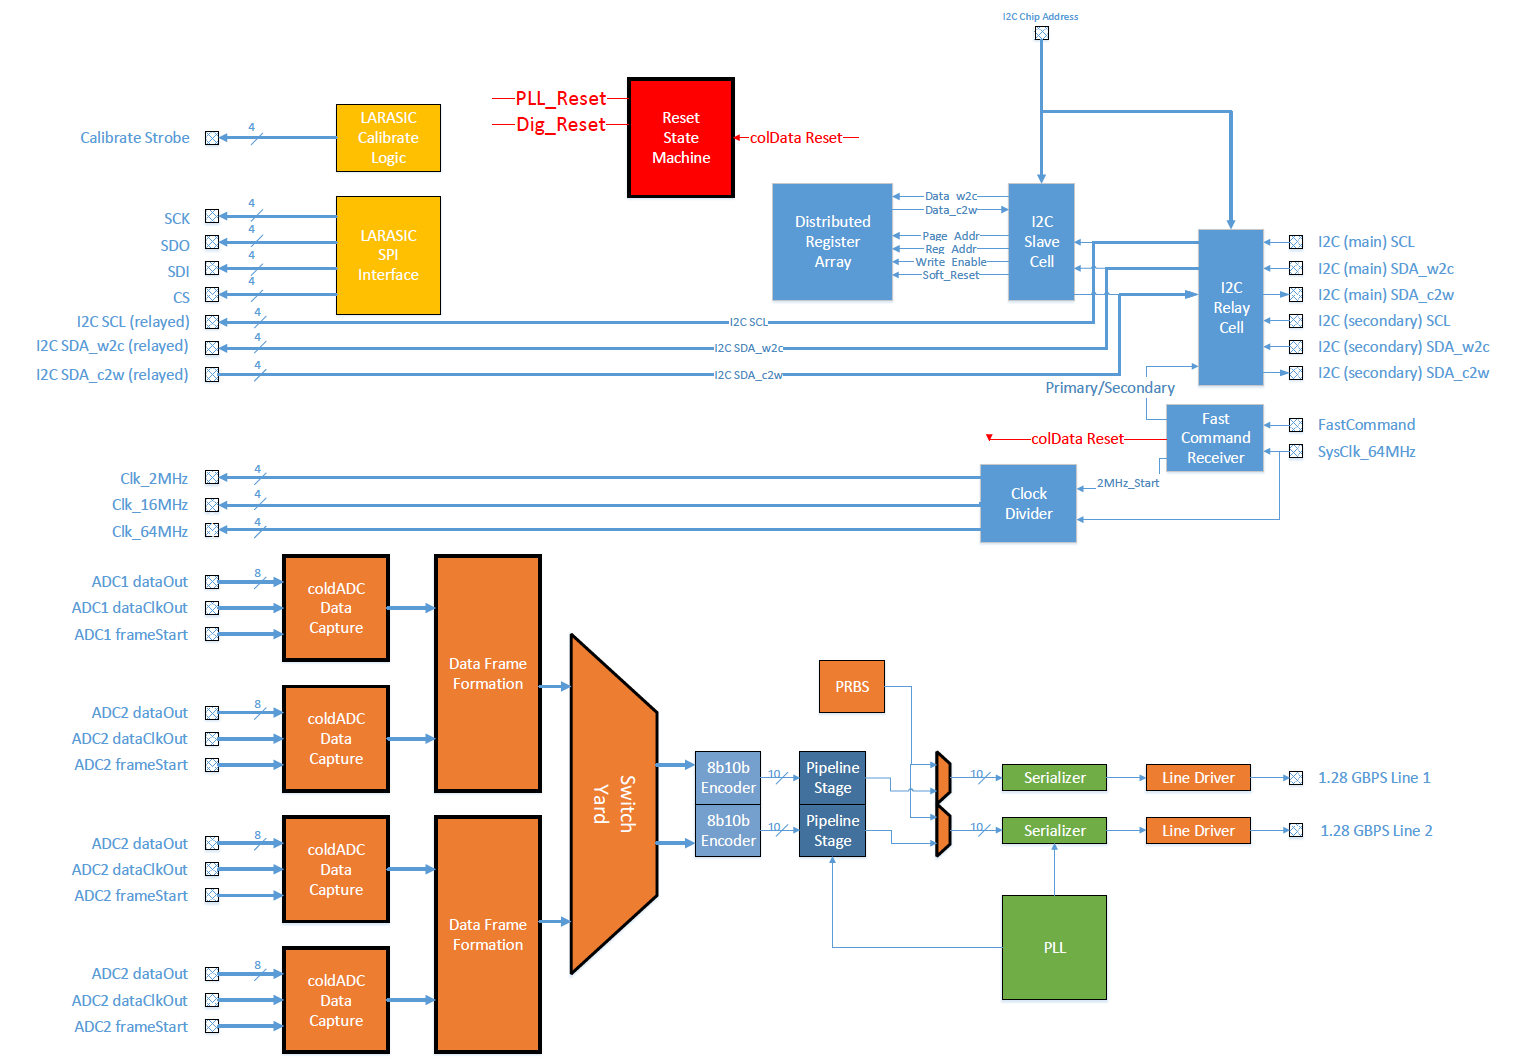
\includegraphics[width=0.85\linewidth]{tpcelec-COLDATABlockDiagram.png}
\end{dunefigure}

Both \dword{coldata} and cold \dword{adc} are implemented in TSMC \SI{65}{nm} \dword{cmos}\footnote{TSMC 65 Nanometer Technology\texttrademark{}, Taiwan Semiconductor Manufacturing Company Ltd., \url{http://www.tsmc.com/english/dedicatedFoundry/technology/65nm.htm}.} 
using cold transistor models produced by Logix Consulting~\footnote{Logix Consulting\texttrademark{} \url{http://www.lgx.com/}}.  Logix made measurements of \fnal-supplied TSMC \SI{65}{nm} transistors at a variety of temperatures (including room temperature and LN$_2$ temperature).  They extracted and provided to \fnal SPICE (Simulation Program with Integrated Circuit Emphasis) models as a function of temperature.  A special library of standard cells, based on these SPICE models and using a minimum channel length of \SI{90}{nm}, was developed by members of the University of Pennsylvania and \fnal groups.  This library was designed to eliminate the risk posed by the hot carrier effect.  The digital sections of \dword{coldata} and cold \dword{adc} use these standard cells and were synthesized from RTL (register-transfer level) using automatic place and route tools.
